% This is LLNCS.DEM the demonstration file of
% the LaTeX macro package from Springer-Verlag
% for Lecture Notes in Computer Science,
% version 2.4 for LaTeX2e as of 16. April 2010
%
\documentclass{llncs}
%
\usepackage{makeidx}  % allows for indexgeneration
\usepackage{graphicx}
\usepackage{caption}
\usepackage{listings}

\lstset{
  captionpos=b,                    % sets the caption-position to bottom
  frame=single,                    % adds a frame around the code
}
%
\begin{document}
\frontmatter          % for the preliminaries
%
\pagestyle{headings}  % switches on printing of running heads
%
\mainmatter              % start of the contributions
%
\title{Optimizing Parallel Dataflows in Software-Defined Networks}
%
\author{David Grigorjan \and Mohammad Hammad \and Robert Oberbeck \and
Nico Scherer \and Maxim Tschumak}
%
\institute{Technical University of Berlin\\
Electrical Engineering and Computer Science\\
Complex and Distributed IT-Systems\\
10623 Berlin, Germany
}
\maketitle              % typeset the title of the contribution

% abstract
\begin{abstract}

To process large amounts of data in an efficient manner, execution is often scheduled in parallel on
multiple nodes. Parallel dataflow frameworks can handle this task but its schedulers currently lack
network awareness. Further, dynamic networking, so called \textit{Software Defined Networking}, is
arising. To improve the efficiency in terms of total execution time of data processing, this paper
presents an approach of coupling the Apache Flink data processing engine with a Software Defined
Network. Different approaches of scheduling tasks to nodes are introduced and discussed. Also, a
middleware is developed that handles topology adjusted execution job placement and network-link load
balancing, leveraging Software Defined Networking capabilities, making data processing overall
faster and more efficient. Deployment on a software-based testbed shows performance gains from this
approach.

\end{abstract}

\keywords{Software Defined Network, Distributed Data Processing}

\keywords{Software Defined Network, Distributed Data Processing,  Apache Flink}
% content
\section{Introduction}
This paper deals with optimizing performance of parallel dataflows in \textit{Big Data Analytics}
utilizing \textit{Software-Defined Networking} (\textit{SDN}). The significance of Big Data
Analytics software stems from the prevailing need of many businesses to process large volumes of
data. However, many of such systems do not consider the network topology they are deployed on.

Throughput and processing time of an analytical program running on distributed clusters can be
improved by utilizing knowledge about the underlying network or managing the network devices
dynamically during runtime. We present some approaches and evaluate one of the more promising among
them.

We test if, how and by what margin advantages of SDN-based environments over traditional ones
increase the performance of a specific data processing engine for use in clusters. We adjust the
scheduler of the engine and develop a middleware that communicates with it as well as with our
network's control component such that information on the network is delivered to the scheduler on
demand.

\section{Data Processing Environment}
For this paper, we used Apache Flink as data processing engine. Flink is a Fast and Reliable
Large-Scale Data Processing engine. A Flink cluster can be made up from a number of physical
computation nodes or even a single host. Processing programs, written in Java or Scala, are
automatically adapted by the optimizer and runtime to execute efficient on a given setup.
\footnote{(2015) Apache Flink home. Retrieved March 20, 2015, from https://flink.apache.org/.}
The result of this adaption is the so-called Execution Graph, which is deployed. A master-node, the
Job Manager is responsible for doing so and keeping track of the the overall job execution. The job
is split up into several tasks that can be handled independant by Task Managers - the actual
computation nodes.  Depending on the physical hardware, a task manager can offer multiple processing
slots. A sketch of the processing is depicted below.

\begin{figure}[h]
    \centering
    \begin{minipage}{0.5\textwidth}
        \centering
        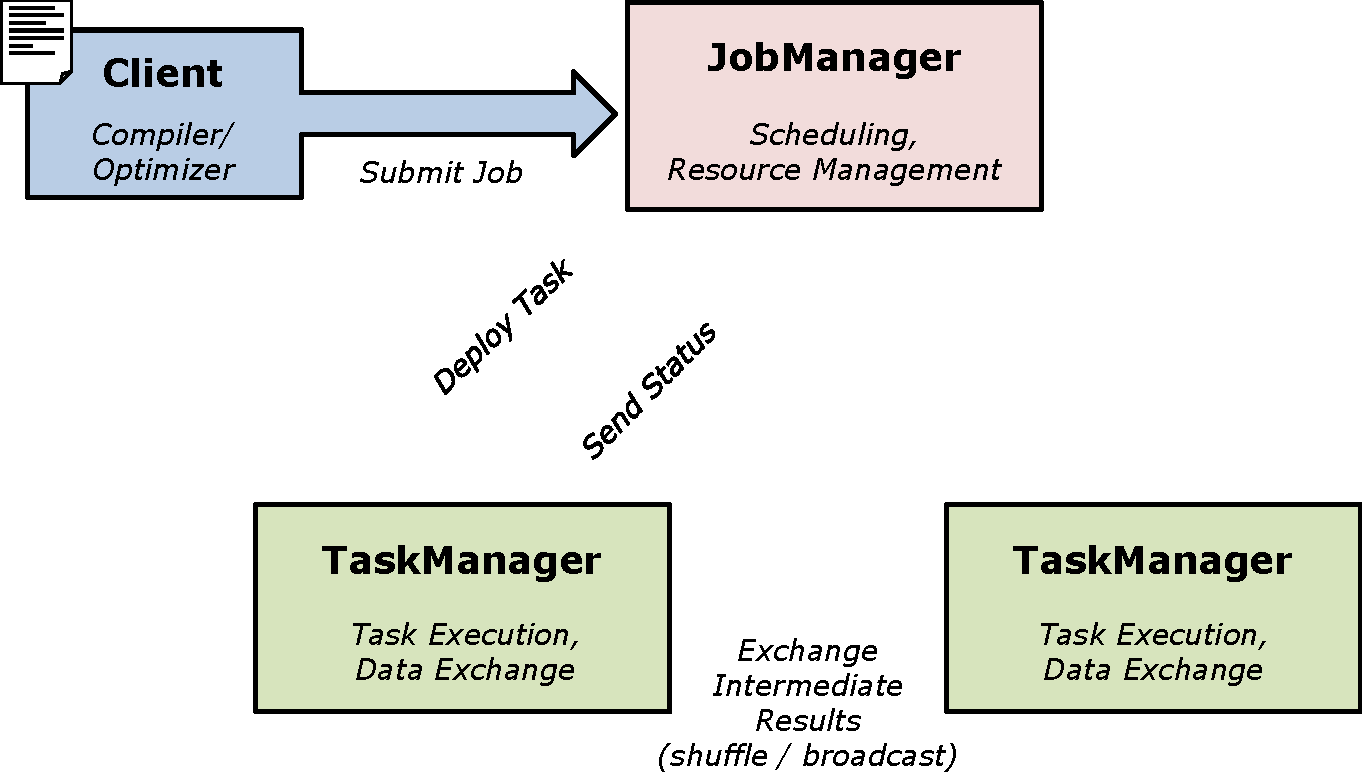
\includegraphics[width=1.0\linewidth]{graphics/ClientJmTm.pdf}
        \captionof{figure}{Sketch of Job Execution\protect\footnotemark}
        \label{fig:job_execution}
    \end{minipage}%
    \begin{minipage}{0.5\textwidth}
        \centering
        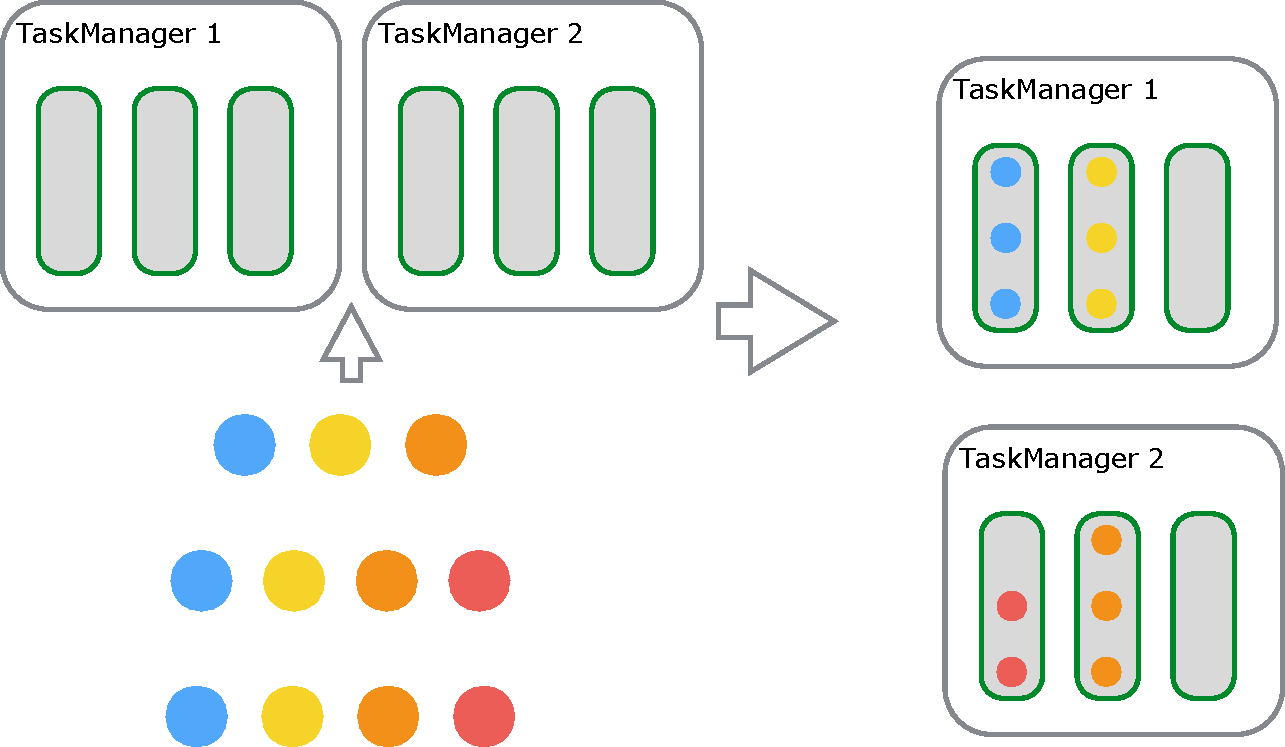
\includegraphics[width=1.0\linewidth]{graphics/slots.pdf}
        \captionof{figure}{Execution-Graph embedding to Task Managers\protect\footnotemark}
        \label{fig:embedding}
    \end{minipage}
\end{figure}

\footnotetext{(2015) ClientJmTm.svg Github/Apache/Flink-master from
https://raw.githubusercontent.com/apache/flink/master/docs/img/ClientJmTm.svg.}

\footnotetext{(2015) Slots.svg Github/Apache/Flink-master from
https://raw.githubusercontent.com/apache/flink/master/docs/img/slots.svg.}


\section{Approach}
To schedule processing tasks on software defined networks, we identified two approaches, which we
named \textit{Top-Down} and \textit{Bottom-Up}. A sketch of these concepts and their relation to the
setup is depicted in Figure \ref{fig:schedulingapproaches} and described in the following section.

\begin{figure}[h]
    \centering
    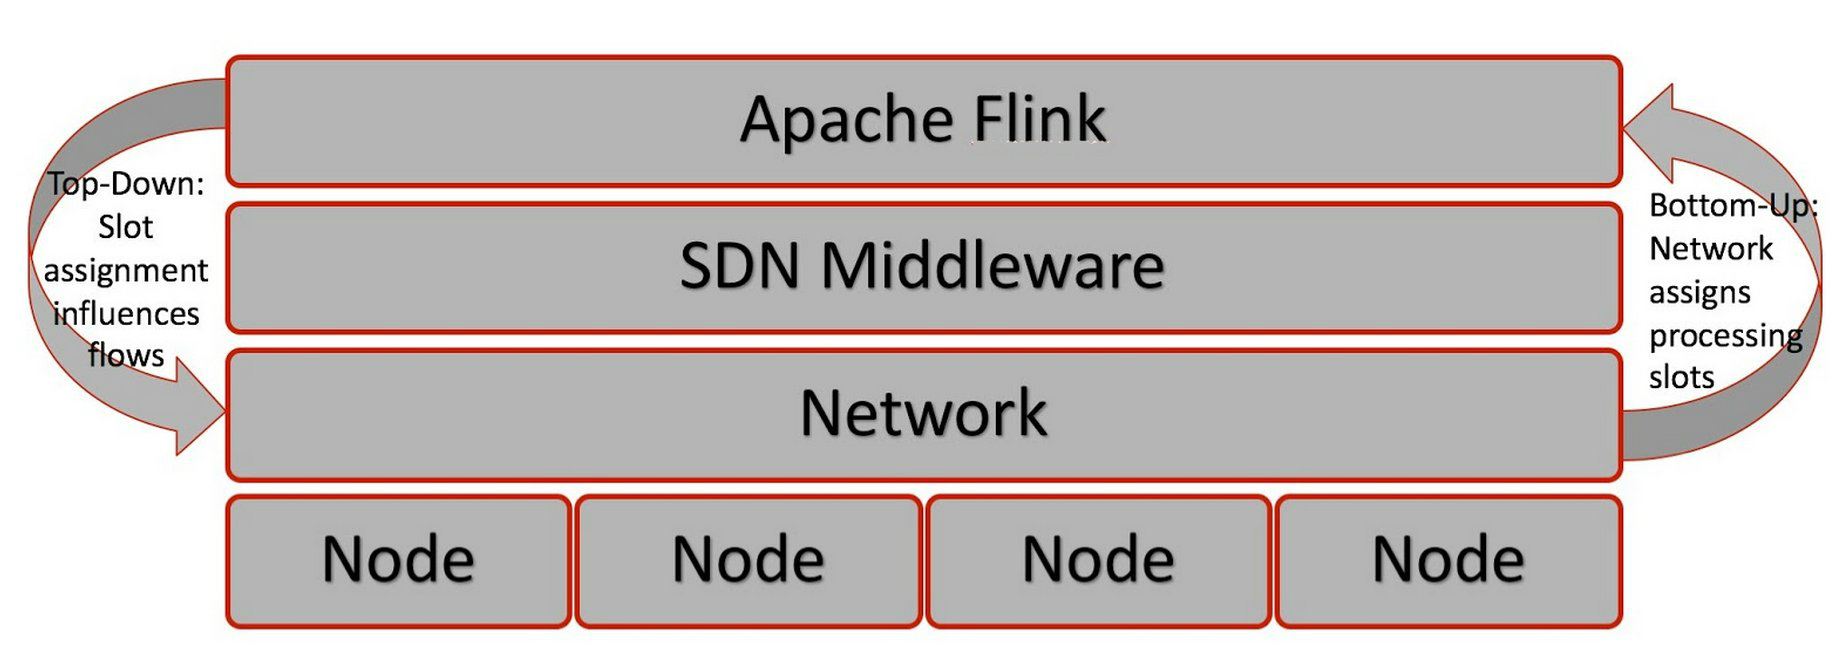
\includegraphics[width=0.75\textwidth]{graphics/schedulingapproaches.png}
    \caption{Different scheduling approaches}
    \label{fig:schedulingapproaches}
\end{figure}

We make the following assumptions:
\begin{itemize}
\item Jobs are not scheduled in parallel but one after another. Otherwise, the scheduler may
interfere with scheduling multiple jobs concurrently.

\item Jobs always communicate All-To-All. This holds true for the experiments conducted within this
paper and eliminates the need to traverse the execution graph. Also, this benefits the generic
approach since no deep Flink requirement is built up and the application can be more easily ported.

\item Due to the fact that network behaviour is to be studied, the focus lies on network
communication. If a single task manager offers multiple processing slots, network effects are
weakened. Therefore, a task manager consists of a single processing slot in our setup.
\end{itemize}

These constraints limit real-world applications but can easily hold true for our test setup to
determine performance gains with the concepts introduced.

\subsection{Top-Down/Flow Switching}
The \textit{Top-Down} approach imposes that the data processing engine schedules tasks as usual and
does not take network properties into account. The middleware is aware of these scheduling decisions
and influences the network properly. This influence could be either providing additional bandwidth
between communicating hosts through flow switching or limiting bandwidth on the specific
communication links for background activities. Advantages of this approach are that there is no
modification on the scheduler required and it is more portable since only a data processing
engine-middleware interface must be implemented. A major disadvantage is the possible worst case:
Parts of a job could be scheduled in a data center and another part far away like in another network
region.

\subsection{Bottom-Up/Scheduling}
The \textit{Bottom-Up approach} required the data processing engines' scheduler actively asks the
middleware for a node to place the task on. The middleware is aware of the network topology and can
determine optimal task placement through proper algorithms. The disadvantage of this approach is
that the data processing engines' scheduler needs to be modified to interact with the middleware.
Advantages would be that the middleware is in full control of job placement what not only ensures
optimal placement but also can add optional constraints like only use certain network areas for
processing during maintenance etc.

A detailed description of the actual implemented algorithms used is given in section
\ref{sec:middleware_slot_assignment}.

\section{Implementation}
To evaluate the approaches described in the previous section, concrete realizations of an SDN
controller and data processing engine is needed. With Apache Flink, the data processing engine
constraint was already given. Besides that, a middleware software has to be implemented as a layer
between network and high level data engine. To achieve the project goals, a middleware has to be
implemented to connect low level network management via SDN controller and high level distribution
of the data processing tasks. We implemented the approaches usind \textit{Apache Flink} and
\textit{OpenDaylight}.

\subsection{SDN Controller}
We use the OpenDaylight (ODL) as our SDN Controller. It features good interoperability as well as
scalability. It communicates via OpenFlow with the virtual switches for routing and forwarding
purposes as well as via a REST-interface with custom programs, acting as a server providing network 
information on demand. 

\subsection{Requirements}
In the previous sections, two approaches have been introduced: scheduling and flow switching.
Implementation of the logic and algorithms relies on some requirements to the middleware software.
These are the summarized requirements:
\begin{itemize}
	\item retrieve information about network topology from SDN controller
	\item host management (scheduling)
	\item load balancing (flow switching) through SDN controller
	\item visualization of current network status
\end{itemize}
First, the middleware has to obtain information about the network topology and its current status.
To get information about the underlying network, a REST client is required to communicate with the
Northbound Topology API of OpenDaylight controller. Another requirement to the specification of the
middleware is realization of the scheduling approach. More specifically, it is the implementation of an
algorithm of how the physical hosts (slots) are assigned to the tasks of the data processing engine.
This should be achieved in a way that the network communication between hosts is efficient and the
network resources are utilized as much as possible. The host assignment should be based on the
information about the network topology and the current status. The Top Down approach tries to
optimize the network utilization during runtime. The middleware needs to have information about the
currently executing job and its deployment (and distribution) in the network. This information is
provided by the data processing engine and should be transferred to the middleware. The middleware
has to analyze the data and optimize data flows by setting network flows through SDN controller. As
an optional requirement, a graphical representation of the current network topology and the host
assignment may be implemented. This functionality can be useful for monitoring, controlling and
debugging of the middleware and the current job execution.

\subsection{Middleware Architecture}

\begin{figure}[h]
    \centering
    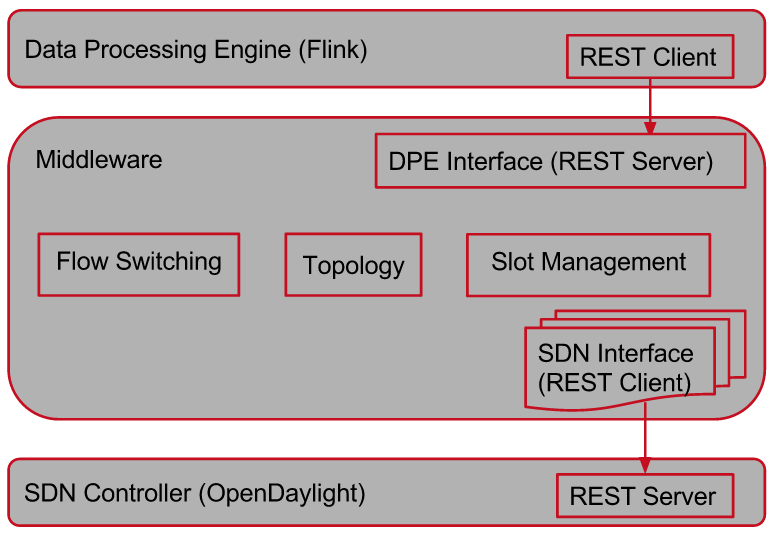
\includegraphics[width=0.8\textwidth]{graphics/architecture.png}
    \caption{Middleware Architecture}
    \label{fig:architecture}
\end{figure}

The architecture of the implemented middleware software is shown in Figure 3.\\
The highest level in the architecture is the data processing engine Flink. After the creation of the
execution graph and before deployment on the hosts, a communication client has been added to the Flink's
scheduler internals to communicate with the middleware. This client sends the execution graph and
requests new hosts for the job as soon as they are needed. The hosts, which finished execution are
released through a call of this client as well. The corresponding server side is a part of the
middleware. \\
The topology module collects all the data about the network: topology (network devices, hosts and
connections between them) and the current utilization of the network. The slot management part is
responsible for slot allocation for the distributed data engine. Algorithms behind it and the generic
API belong to this module as well. \\
The flow switching module takes care about the optimization of the network flows based on the
current execution graph and network status. In order to access the Northbound API of the SDN
controller, generic interfaces were defined so that the middleware does not depend on one particular
implementation of a SDN controller. The concrete realization of northbound clients was done
separately for the required APIs, such as Flow Programmer and Topology API.\\
The network visualization module was implemented as well as part of the middleware.\\
Technically, the middleware is implemented as a Maven multi module project. This decision was made to
take advantage of the benefits of a structured project powered by a feature rich build system: flexibility,
customizability, dependency management, task automation and more. All the algorithms are covered
with tests and the source code is published under Apache License\footnote{(2015). Distributed
Systems Master Project WS14/15 ∙ GitHub. Retrieved March 12, 2015, from https://github.com/citlab/vs.msc.ws14}.

\subsection{Middleware Slot Assignment}
The I/O operations are often the bottleneck of distributed data processing setups\cite{cheating}. Besides
reading and writing to disk, there is the communication layer over the network. The Bottom Up
approach should help to organize the execution slots in a way that they are able to communicate in an
efficient manner over the network. In this section, the algorithm for  slot distribution over the
network is described.

\begin{figure}
    \centering
    \begin{minipage}{0.5\textwidth}
        \centering
        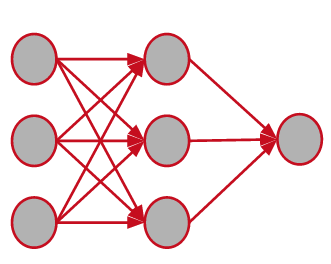
\includegraphics[width=0.6\linewidth]{graphics/executiongraph.png}
        \captionof{figure}{Execution graph}
        \label{fig:execution_graph}
    \end{minipage}%
    \begin{minipage}{0.5\textwidth}
        \centering
        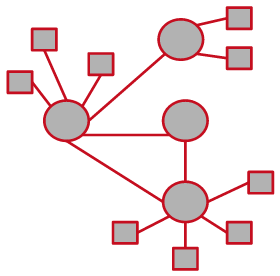
\includegraphics[width=0.6\linewidth]{graphics/topology.png}
        \captionof{figure}{Network Topology}
        \label{fig:network_topology}
    \end{minipage}
\end{figure}

As a starting point, there is the execution graph (Figure \ref{fig:execution_graph}) and the network
topology (Figure \ref{fig:network_topology}).  This information derives from data processing engine
and SDN controller respectively. Besides that, it is possible to collect data about the current
utilization of the network over the SDN controller.  The execution graph represents the steps of the
job execution and the network topology is a formation of hosts, network devices and links between
them in the network. Both of them are directed graphs. The question is how to map one graph
into another to achieve the best links between the executors.

The general approach is to find an isomorphism between the two graphs. But first, the execution
graph has to be normalized since Flink (and other data processing engines) will more likely execute
some of the nodes of execution graph on the same physical host (or even on the same slot). Because
of this, the normalization function of the graph depends strongly on the engine being used, so this
solution would be not generally applicable. Furthermore, there are no efficient algorithms available
resolving this problem (graph isomorphism problem) and the complexity of it is even unknown \cite{graph}.

Another reasonable approach is the solution to the general heaviest k-subgraph problem. Using the
algorithms to calculate the heaviest subgraph it is possible to get k nodes of the graph which
connections have the biggest weight. Data processing engine’s deployments of the tasks are not
static and can be made during runtime. Because of this, there is no information about the total
number of hosts (slots) needed for the complete run and the solution to the heaviest k-­subgraph
problem cannot be applied to the process engines with dynamic deployments. Besides this, the
algorithm is NP­-hard by reduction from the clique problem and does only work for undirected graphs
\cite{ksubgraph}.

It was not possible to find an optimal solution based on known theoretical approaches. Therefore, a
custom approach has been developed and implemented. Intuition for the algorithm is that
all hosts which are directly connected to the same switch (general: network device) may have better
links than hosts connected through more than one switch. The number of hubs and link “quality” also
affect the transference of the data.

\begin{figure}[h]
    \centering
    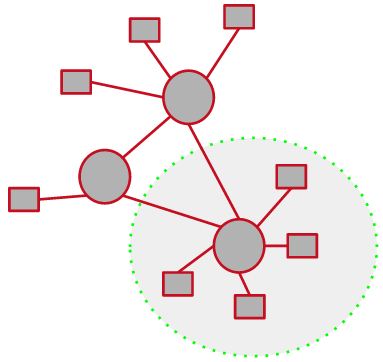
\includegraphics[width=0.4\textwidth]{graphics/hostgroup.png}
    \caption{HostGroup in network topology}
    \label{fig:hostgroup}
\end{figure}

First, we define a \textit{Host Group}. A network device (circle in Figure \ref{fig:hostgroup}) and all
directly connected hosts (rectangles in Figure \ref{fig:hostgroup}) constitute a Host Group.
Thus, network topology consists of a set of Host Groups and each of them consists of one switch and
a set of hosts. Furthermore, we define the quality of the link between the hosts by affiliation of
the hosts to the same Host Group.

\begin{equation}
    weight\_full = data\_size / (bandwidth - bandwidth\_used) + latency
\end{equation}
\begin{equation}
    weight\_simple = data\_size / bandwidth
\end{equation}

If two hosts are not in the same Host Group, the quality of the connection between them is the
transmission time for the data needed to be sent between the switches of the two Host Groups where
the hosts belong to. This value weight of the edge in the topology graph is used to calculate the
shortest paths by the Dijkstra algorithm. In case there are no statistics about current utilization
of the network, a default size can be applied.\\

\begin{lstlisting}[caption=Algorithm of finding free hosts based on Host Group concept]
IP: findNextBestHost()
    if no_free_hosts()
        return NULL
    if all_hosts_are_free()
        return get_biggest_host_group().getFreeHost()
    if working_host_group_has_free_hosts()
        return free_host_group.getFreeHost()
    else
        return next_best_host_group().getFreeHost()
end
\end{lstlisting}

The algorithm in pseudocode is shown in Listing 1. Basically, there are only four options. If
there are no free hosts available, the data process engine will not get any host for its
calculations. In case that all hosts are free, the biggest Host Group will be selected and the data
processing engine receives one of the host for executions. If there is a Host Group with some
occupied and idle hosts, one idle host will be returned to the data processing engine. In the last
case, there are some Host Groups which are fully occupied. In order to find the next best Host
Group, the algorithm searches for the Host Group with the best link to the Host Groups that is
currently occupied using shortest paths calculated by Dijkstras’ algorithm.

The implementation of this concept and algorithms is thread safe and optimized to be efficient
(caching). Furthermore, the algorithms can be easily adapted to execute different parallel jobs on
the same topology at the same time.

\subsection{Future Work}
\subsubsection{Traffic Properties}
Monitoring would be an enabler for better scheduling and flow programming, by taking latency and
network utilization into account.

The OpenFlow specification \cite{openflow} offers port- and flow-based packet- and byte-counters,
but neither is measures latency nor bandwidth. Therefore monitoring has to be somehow implemented.
One approach to determine latency between two switches is to insert additional packets and measure
the duration. The PACKET OUT and PACKET IN functions of OpenFlow would be used. PACKET OUT messages
forward additional packages to one or more ports. The payload of this message is the timestamp of
its creation. The OpenFlow controller receives a PACKET IN message when a switch could not assign a
packet to a flow of its flow table. The latency can then be easily calculated by subtracting the
time of packet creation and roundtrip times from the time the packet was received via PACKET IN. The
roundtrip times can be measured by sending a packet to a switch, which is returned immediately.
\cite{monitoringlatency} \cite{opennetmon}

OpenFlow also supports a FLOW REMOVED message that is received by the controller when a flow entry
of a switch is expired since every flow entry exists only for a certain period of time. This message
contains information about the duration an entry was active in the flow table, the amount of traffic
matched against an entry and the input port to determine the source of traffic. These information
enable the computation of utilization between inter-switch links. This approach does not produce any
instrumentation overhead since the FLOW REMOVED messages are send anyhow. A drawback might be that
the information are only available for the point of time when the flow was removed. \cite{flowsense}

Another way to measure network utilization is to poll the OpenFlow statistics. Fetching the
statistics of a switch causes some overhead, therefore the problem is to find an intelligent polling
algorithm to reduce the load on switches. Using the routing information of a flow is helpful to find
an appropriate querying strategy. The switch closest to the destination offers the most accurate
statistics but there would be a huge load on this switch. While querying a switch randomly has
better load balancing but is less accurate. A good compromise is to query two switches randomly and
select the one closer to the destination. \cite{opentm} \cite{opennetmon}

There are implementations for the OpenFlow Controller POX \cite{opennetmon}, NOX \cite{opentm} and
Floodlight \cite {flowsense}.

\subsubsection{Loadbalancing}
Even using the Bottom Up approach, the possibility to control data flows in the network still
remains. The notion of balancing data flows of alike source and sink around multiple paths comes to
mind. OpenDaylights’ default flow configuration behavior is handled by an interchangeable part
application titled Simple Forwarding. Upon activation by a switch clueless how to reach a packets’
destination, the application prompts the updating of all switches connected to the controller so
that future packets to the said destination host will follow along the shortest path. This behavior
might be sufficient in the case where sources and sinks are not grouped around common switches but
in our case we would have lots of tasks deployed on host groups characterized by single switch
connections due to our scheduling decisions. In the assumed case of all-to-all data-flows between
two or more host groups, we would not want to send all data along a single path. Even with the
switch of each host group posing as a natural bottleneck, we assume better overall load balancing
would stem from using more than a single shortest path which we could determine with Yen’s
Algorithm.

\section{Test Setup}
The Flink Cluster was built on a single physical host using virtualization and the SDN simulator
Mininet.

\subsection{Mininet}
Mininet is a software to simulate SDN environments on local machines. It  emulates physical hosts,
switches, links and routers on a Linux Kernel. \footnote{(2012). Introduction to Mininet ∙
mininet/mininet Wiki ∙ GitHub. Retrieved March 12, 2015, from
https://github.com/mininet/mininet/wiki/Introduction­to­Mininet} For topologies, either built-in or
shipped-with ones can be used or one can create custom topologies. Connected hosts are isolated from
each other and behave like real ones. For emulating switches, Mininet uses
Open-vSwitch\footnote{(2009). Open vSwitch. Retrieved March 12, 2015, from
httop://openvswitch.org/}, a virtual switch emulation software, controlled by OpenFlow.

With Mininet modeling all physical properties of a real SDN environment, ordinary network
diagnostics and manipulation software can be used. Also, Mininet is able to use a variety of SDN
controllers. The built-in one is based on POX but external ones can be connected by providing the
corresponding IP address and port number. For this work, we used the external controller option and
connected Mininet to an OpenDaylight controller.

Since the Mininet-network is emulated in an isolated environment, connected hosts do not have access
to the outer world, e.g. the Internet. To establish a connection, a Network Address Translation
Router (NAT) has to be connected. This is required to be able to communicate between cluster nodes
and the middleware.

\subsubsection{Typical Network Topology}
To evaluate the performance gain using the approach described in this paper, we need to create a
topology that resembles currently deployed network infrastructures at data centers as close as
possible. A common network structure is the so-called Fat Tree. \cite{datacenter} This topology
connects hosts and switches in a tree-like manner, with hosts on the lowest layer and switches in
the layers above.  Since link bandwidth increases with higher layers, the tree is called fat. A
sketch of this setup is depicted in the image below.

\subsection{System properties}
The test setup was built on a single physical host. Its physical properties are listed in the table
below.

\begin{table}[h]
    \centering
    \begin{tabular}{| l | l | }
        \hline
        \textbf{Property} & \textbf{Value} \\ \hline
        Operating &  System Windows 8.1 x64 \\ \hline
        CPU Intel & Core-i7 3720QM \\ \hline
        Memory & 8GB 1600MHz DDR3 \\ \hline
    \end{tabular}
    \caption{Physical host properties}
    \label{table:host_properties}
\end{table}

On top of the physical host, we implemented a virtualized testbed with the following properties.

\begin{table}[h]
    \centering
    \begin{tabular}{| l | l | }
        \hline
        \textbf{Property} & \textbf{Value} \\ \hline
        Virtualization software & VMWare Player 6.0.4 \\ \hline
        Operating System & Ubuntu 14.10 x64 \\ \hline
        Number of CPUs & 4 \\ \hline
        Memory & 5100MB \\ \hline
        Mininet & version 2.2.0rc2 \\ \hline
        Open vSwitch & version 2.1.3 \\ \hline
        OpenDaylight & version 0.2.2-SR2 \\ \hline
        Flink version & 0.7.0 incubating \\ \hline
    \end{tabular}
    \caption{Virtualized guest properties}
    \label{table:guest_properties}
\end{table}

Within the virtual guest, a mininet environment was built up with the topology described in the
mininet section of this paper. A Flink cluster was configured to handle every node as worker and use
128MB of heap per taskmanager. Further, a DoP of 5 was set. For all links, packet loss was set to 0\%
and delay to 2ms. Bandwidth was set to 5, 10 or 20MBit/s, depending on the link layer.

\subsection{Evaluation}
To evaluate the performance gain of our modified Flink setup, we compared job execution times of the
unmodified, native Flink application versus our SDN implementation. For KMeans, we used 5000
datapoints and a variable number of clusters and iterations. The results are shown in the following
table.

\begin{table}[h]
    \centering
    \begin{tabular}{| l | l | l | l | l | }
        \hline
        \textbf{No of Clusters} & \textbf{Iterations} & \textbf{Execution time}
            & \textbf{Execution time} & \textbf{Speedup in \%} \\
        & & \textbf{native in s} & \textbf{modified in s} & \\ \hline

        5 & 10 & 16.823 & 17.587 & -4.54 \\ \hline
        5 & 100 & 38.042 & 27.367 & 28.08 \\ \hline
        50 &10 &15.195 &9.689 &36.24 \\ \hline
        50 &100 &35.46 &19.979 &43.66 \\ \hline
        500 &10 &13.072 &9.166 &29.88 \\ \hline
        500 &100 &50.547 &24.378 &51.77 \\ \hline
    \end{tabular}
    \caption{Results of evaluation}
    \label{table:guest_properties}
\end{table}

As one can see, the implemented approach results in an overall speedup of the computation, merely
one configuration resulted in a performance decrease. It is remarkable that we gain up to 51.77%
performance increase despite the fact that additional roundtrips are required for asking the
middleware for hosts to place the task on.


%references
\nocite{*}
\bibliographystyle{splncs03}
\bibliography{bibliography}

\end{document}
